

\subsection{Candidate Picker}
\label{sec:picker}

%  clean the page need to make it clear and normalized.  So we preprocess
% all the tree nodes in the following several aspects.

% \begin{itemize}
%   \item \textbf{Filter unwanted nodes}:
%   We will remove all the comment nodes in the DOM tree
%   since they are nothing to do with the actual page rendering. In addition, we keep a black list of tags which are unlikely to contain a top-$k$ list.
%   %such as \emph{$<$head$>$, $<$link$>$, $<$style$>$, $<$form$>$ $<$iframe$>$} and so on.
%   %We list those tag names in Table \ref{tab:blackTag}.
%   \item \textbf{Combine adjacent siblings}:
%   In some cases, two adjacent tag nodes may be of the same tag name. For some particular tags, such as {\tt <strong>} and {\tt <i>} we can move the the child nodes of the latter node into the former and remove the latter node, i.e., combine the two nodes together. This replacement will not affect the display effect and make the tree clearer. However this does not work for all the tags, for example, if we combine two adjacent ``h1'' tags, the rendering of the page will be changed.
%   \item \textbf{Handle image tags}:
%   Our system is originally designed to extract text node lists.
%   Later we find that images are also useful to describe list items, for example the third column in Table \ref{tab:sampleoutput}.
%   In order to make the system compatible to image tag nodes, we can replace a image node with a text node, the content of which is specified by the image URL. Therefore, we can extract image lists just like other normal lists and then retrieve the images by the URLs.
% \end{itemize}



This step extracts one or more list structures which appear to be top-$k$ lists
from a given page.
%Given a top-$k$ page, we want to find candidate lists from the
%page. We use an HTML parser to parse the page into a DOM tree, and
%then we perform some necessary cleaning.
%
A top-$k$ candidate should first and for most be a list of $k$ items,
Visually, it should be rendered as
$k$ vertically or horizontally aligned regular patterns.
While structurally, it is presented as a list of HTML nodes with
identical \emph{tag path}.
A \emph{tag path} is the path
from the root node to a certain tag node, which can be presented as
a sequence of tag names.  Figure \ref{fig:tagpath} shows the relation
between list nodes and tag paths.

\begin{figure}[th]
\centering
\epsfig{file=pics/tagpath.eps,width=0.9\columnwidth}
\caption{List Nodes and Their Tag Paths}
\label{fig:tagpath}
\end{figure}


%For extraction of top-$k$ lists, we notice that items in a top-$k$
%list usually have similar format and style, and therefore they often
%share an identical \emph{tag path}.  A \emph{tag path} is the path
%from the root node to a certain tag node, which can be presented as
%the concatenation of tag names.  For example, in Table
%\ref{tab:sampleoutput}, the tag path corresponding to the second
%column {\em Name} is {\tt html/body/.../div/h2}.

Based on these observations, the system employs two basic rules for
selecting candidate lists:
\begin{itemize}
  \item \textbf{K items}:
  A candidate list must contain exactly $k$ items.

  \item \textbf{Identical tag path}:
  The tag path of each item node in a candidate list must be the same.
\end{itemize}

The \emph{Tag Path Clustering Method}, shown in
Algorithm~\ref{algo:tagPath}, process the input page according to the
two basic rules. Inspired by Miao et al.\cite{MiaoTHSM09:TagPathClustering}, the algorithm
recursively computes the tag path for each node (Line 2), and groups
text nodes with identical or very similar tag path into one node list. 
When this procedure completes, we get a set of node lists, those of which
with precisely $k$ nodes are selected into the candidate set.

%
%\begin{enumerate}
%  \item \textbf{Compute the tag path for each node}:
%  We can traverse the DOM tree and get the tag paths for all nodes.
%  The tag path of a node $n$ can be calculated recursively by concatenating its parent's tag path
%  with its tag name and a splitter.
%  The splitter is a constant string which serves as boundaries between tag names in the tag path.
%  Since we need to know the tag path of the parent node before the calculation
%  the traversal is done in a preorder manner.
%
%  \item \textbf{Group text nodes with an identical tag path}:
%  After computing the tag path we have a mapping from a node to a tag path string. Then we want the reverse mapping,
%  which is from a tag path to a list of nodes that share the tag path. We can use a hash table as the data structure, of which the key type is string and value type is list of node.
%  We can traverse all the text nodes and for each node $n$,
%  we insert itself to the node list that is corresponding to $n$'s tag path in the hash table
%  (if the table does not contain $n$'s tag path as key yet, insert the tag path with a value of a new empty list into the table).
%
%  \item \textbf{Select $k$-item lists}:
%  With a table of node lists of equivalent tag paths(as keys), we select those node lists of $k$ items (i.e, $k$ text nodes).
%  We consider them as candidate lists.
%\end{enumerate}
%
%We can put the first and second step together in one traversal, which is shown in Algorithm \ref{algo:tagPath}.

\begin{algorithm}
\caption{Tag Path Clustering Method}
\label{algo:tagPath}
\begin{algorithmic}[1]
\Procedure{TagPathClustering}{$n$,$table$}
%\Comment The current node, $n$; \\
%\Comment The hash table of node lists, $table$ ; \\
\State $n.TagPath \gets n.Parent.TagPath+Splitter+n.TagName;$
%\Comment Calculate the tag path of $n$
\If {$n$ is a text node}
    \If{$table$ contains the key $n.TagPath$}
        \State  $list \gets table[n.TagPath]$;
    \Else
        \State  $list \gets$ new empty lists;
        \State  $table[n.TagPath] \gets list$
    \EndIf
    \State  Insert $n$ into $list$;
    \State \textbf{return};
\EndIf
\For{each node $i \in n.Children$}
%    \IF{$i$ is a tag node}
    \State $TagPathClustering(i,table)$;
%    \ENDIF
\EndFor
\State \textbf{return};

\EndProcedure
\end{algorithmic}
\end{algorithm}

%
%With the two rule, a.k.a the \emph{Default} rule,
%we can pick all satisfactory lists and build a \emph{Default} candidate set.
While the above method harvests most top-$k$ lists (with high recall),
it also produces many false positives.
%The basic algorithm often produces too many noise lists and reduce the precision of the whole system.
We thus introduce three additional pattern-based rules to further filter
the candidate lists:

\begin{enumerate}
\item \textbf{Index}:
There exists an integer number in front of every list item, serving as
a rank or index: e.g., ``1.'', ``2.'', ``3.'', etc.
Moreover, the numbers are in sequence and within the range of
$[1, k]$ (e.g., Figure \ref{fig:indexPattern}).

\item \textbf{Highlighting Tag}:
The tag path of the candidate list contains at least one tag
among {\em $<$b$>$,$<$strong$>$,$<$h1-h6$>$} for highlighting purposes
(e.g., Figure \ref{fig:highlightPattern}).

\item \textbf{Table}:
The candidate list is shown in a table format(e.g., Figure \ref{fig:tablePattern}).
\end{enumerate}

\begin{figure}[th]
\centering
\epsfig{file=pics/indexPattern.eps,width=0.8\columnwidth}
\caption{A Sample List of Index Pattern\cite{Top20Books}}
\label{fig:indexPattern}
\end{figure}

\begin{figure}[th]
\centering
\epsfig{file=pics/highlightPattern.eps,width=0.8\columnwidth}
\caption{A Sample List of Highlight Pattern\cite{highlightPattern}}
\label{fig:highlightPattern}
\end{figure}

\begin{figure}[th]
\centering
\epsfig{file=pics/tablePattern.eps,width=0.8\columnwidth}
\caption{A Sample List of Table Pattern\cite{tablePattern}}
\label{fig:tablePattern}
\end{figure}

%In this modified algorithm, a.k.a. {\em Def+Patt} algorithm,
%We call the three rules above extended rules.  We only accept
Only those lists that satisfy at least one of additional rules
gets to stay in the candidate set. For
example the top-$k$ list in Figure \ref{fig:dotNet}
satisfies rules Index and Highlighting Tag.


\begin{table*}[th]
\centering
\caption{Main Features Used in the Model}
\begin{tabular}{|c||c|c|c|c|}
\hline
Name & Type & Description & Positives & Negatives\\\hline
Word & Boolean & Existence of a certain word in the list text & Indexes (e.g., ``25.'', ``12.'') & ``Contact Us'', ``Privacy Policy''\\
Tag Name & Boolean & The tag name of the list nodes & $<$h2$>$, $<$strong$>$, ... & $<$input$>$,$<$iframe$>$\\
Attribute & Boolean & Existence of a attribute token in the list nodes & ``articleBody'', ``main''& ``comment'', ``breadcrumb''\\
Word Count & Integer & The average word count of the list items& / & / \\
Length Variance & Float & The standard variance of the lengths of the list items & / & / \\
\hline
\end{tabular}
\label{tab:featureType}
\end{table*}

\subsection{Top-K Ranker}
\label{sec:ranker}

Top-K Ranker ranks the candidate set and picks the top-ranked list as the
top-$k$ list by a scoring function which
is a weighted sum of two feature scores below:

%So far, we have managed to build the ranker within two different frameworks,
%which we will discuss respectively.

%\subsubsection{Rule Based Ranker}
%In this framework, we rank each candidate with a score.
%The one with the highest score will be selected as the result.
%To calculate the score, we set a few criteria as follows:

\begin{itemize}
\item \textbf{$P\textnormal{-}Score$}: $P\textnormal{-}Score$ measures
  the correlation between the list and title.  In Section
  \ref{sec:title}, we extract a set of concepts from the title, and
  one of them is the central concept of the top-$k$ list.
  Our key idea is that one or more items from the main list should be
  instances of that central concept from the title. For
  example, if the title contains the concept ``scientist'', then the
  items of the main list should be {\em instances} of the
  ``scientist'' concept. The Probase taxonomy provides large number of
  concepts and their instances. 
 % which were extracted from the web corpus. 
  For instance, the ``scientist'' concept has 2054 instances
  in Probase.

  We calculate the $P\textnormal{-}Score$ of each candidate list $L$
  by:
\begin{equation*}\label{equ:pScore}
  P\textnormal{-}Score= \frac{1}{k} \sum_{n \in L} \frac{LMI(n)}{Len(n)};
\end{equation*}
where $LMI(n)$ is the word count of the longest matched
instance in the text of node $n$,
while $Len(n)$ means the word count of the entire text in node $n$.

%Form Equation we can see that, the $P\textnormal{-}Score$ of a list
%is the average of the ``$P\textnormal{-}Score$''
%($\frac{LMI(n)}{Len(n)}$) of each node.
We divide $LMI(n)$ by $Len(n)$ to normalize the P-Score to $[0,1]$, and
the contribution of each node will be no more than $1/k$,
which makes sure that one single node's effect doesn't dominate the whole
score. In addition, $P\textnormal{-}Score$ prefers lists
with fewer words, because nodes with many words (e.g., a description paragraph)
are less likely to be part of a top-$k$ list.

\item \textbf{$V\textnormal{-}Score$}: $V\textnormal{-}Score$
  calculates the visual area occupied by a list, since
  the main list of the page tends to be larger and more
  prominent than other minor lists.  The $V\textnormal{-}Score$ of a
  list is the sum of the visual area of each node and is computed by:
\begin{equation*}\label{equ:vScore}
Area(L)= \sum_{n \in L} (TextLength(n)\times FontSize(n)^2).
\end{equation*}

 % \item \textbf{$Bonus$}:
%
%  With $bonus$, we can import heuristic rules to the ranking system. Note that bonus can also be negative, which is actually penalty.
%
%  For example, we want to show priorities to the lists that matches the three patterns(index, highlight and table), so we give them a large positive bonus. On the contrary, nodes in some list contain negative attribute values such as ``sidebar'' or ``comment'',
%  which imply the list a non-top-$k$ list. We should assign them a negative bonus.
\end{itemize}


%The final score $F\textnormal{-}Score$ can be calculated by Equation \ref{equ:fScore}:
%
%\begin{equation}\label{equ:fScore}
%    F\textnormal{-}Score(L)= \lambda F\textnormal{-}Score(L)+ \mu V\textnormal{-}Score(L)+Bonus(L);
%\end{equation}
%
%where $\lambda$ and $\mu$ are weights for each criteria.
%

\ZZX{
The above described approach, known as {\em rule-based} ranker
is fairly simple and performs reasonable well.
Its main drawback is that it is based on only two features and
lacks flexibility and extensibility.
%The ranker described above gives good performance. However, it has
%one drawback, which is that it lacks extensibility.  When adding a new
%feature to this framework, we need a lot of experiments to justify
%that it is beneficial to the ranker and also we need to adjust all the
%weights for the features.
We hence propose a {\em learning-based} ranker as a major improvement.
In this new approach,
a Bayesian model is learned from a large training set of candidate lists,
where top-$k$ lists are labeled. The
set of features we use in the model are included in Table
\ref{tab:featureType}, all of which can be automatically extracted
from the given list.
Then we use discretization method to handle numerical feature types (e.g. word count).
For a candidate list, the model generates all
the features and gives the likelihood of positive (top-$k$) and
negative lists with the following equation.
\begin{equation*}\label{equ:likelihood}
P(C|F)=\frac{P(F|C)P(C)}{P(F)} \propto p(C)\prod_{i=1}^{n}p(f_{i}|C).
\end{equation*}
in which, $C \in \{positive, negative\}$,
$F=\{f_{1},...,f_{n}\}$ is the set of observed feature values for the given candidate
and $p(C)$ and $p(f_{i}|C)$ are estimated
with relative frequencies from the training set.
We then normalize $P(positive|F)$ and $P(negative|F)$ into one value and therefore choose
the candidate list that attains the highest probability.}

Compared to the rule-based method, this framework is more flexible
as new features can be added any time. One just need to provide a function
for extracting the new feature values from a list and update the model.
The learning-based ranker can also use $P\textnormal{-}Score$ and
$V\textnormal{-}Score$ as features, so it is strictly more general
than the rule-based approach.
%On the other hand, we can also improve the model using a larger training set.

\subsection{Content Processor}

After getting top-$k$ list, we extract attribute/value pairs for each
item from the description of the item in the list. The goal is to
obtain structured information for each item such as in
Table~\ref{tab:sampleoutput}.  As another example, Table
\ref{tab:rawList} shows a fragment of a top-$k$ list ``Top 100
newspapers in the united states for 2010''.  Content Processor
transforms it into Table \ref{tab:processedList}.  Furthermore,
by analyzing the title, we obtain valuable information like
the \emph{location} is ``the united states'' and
the date is ``2010''. We describe three major steps in the
content processor.

\begin{table}[th]
\centering
\caption{The raw result of a top-$k$ list fragment\cite{top100Newspapers}}
\begin{tabular}{|l|}
\hline
USA Today (Arlington, Va.)\\
Wall Street Journal (New York, N.Y.)\\
Times (New York, N.Y.)\\
Times (Los Angeles)\\
Post (Washington, DC)\\
Tribune (Chicago)\\
Daily News (New York, N.Y.)\\
Inquirer (Philadelphia)\\
Post/Rocky Mountain News (Denver)\\
\hline
\end{tabular}
\label{tab:rawList}
\end{table}

\begin{table}[th]
\centering
\caption{The processed result of a top-$k$ list fragment\cite{top100Newspapers}}
\begin{tabular}{|l|l|}
\hline
\textbf{Newspaper} & \textbf{American city}\\ \hline
USA Today &Arlington, Va.\\
Wall Street Journal &New York, N.Y.\\
Times &New York, N.Y.\\
Times &Los Angeles\\
Post &Washington, DC\\
Tribune &Chicago\\
Daily News &New York, N.Y.\\
Inquirer &Philadelphia\\
Post/Rocky Mountain News &Denver\\
\hline
\end{tabular}

\label{tab:processedList}
\end{table}


\subsubsection{Infer the structure of text nodes}
In many cases, the text node that describes each item may have some inner
structure, or is semi-structured.  For example, the inner structure of
every list item in Table \ref{tab:rawList} is ``XXX(YYY)''. This structure
means the text actually contains multiple columns (and often difference types) 
of information.
%The inner structure enables an HTML node to contain multiple types of
%information, which can be explicitly divided into multiple fields.

We infer the inner structure of the text by constructing the frequency
distribution for each potential separator tokens such as ``By'', ``:'' and
``,'' from all the items of the top-$k$
list \cite{Fisher08:dirttoshovels}.
%The x-axis represents the
%occurrence number of a separator in a node, while the y-axis means the
%number of nodes.
If we identify a sharp spike in the distribution for a
particular token, which means the number of occurrences for that token
is identical among all the list nodes, then we find a separator,
which can be used to separate the text into multiple fields. Each field
is often an attribute or property of the entity described by the list item.
The frequency distribution of various tokens and their occurrences
with a list element in Table \ref{tab:rawList} is shown
in Figure \ref{fig:histogram}
and clearly indicates that the bracket token is a good candidate for
separator.

\begin{figure}[th]
\centering
\epsfig{file=pics/innerstrucutre.eps,width=0.7\columnwidth}
\caption{The frequency distribution of various tokens in the list of Table \ref{tab:rawList}}
\label{fig:histogram}
\end{figure}


\subsubsection{Conceptualize the list attributes}
Once the list items are broken down into attribute values, it is useful
to infer a {\em schema} for these attributes.
%It is important to provide names (types) to the extracted attribute
%values.
For example, in Table \ref{tab:processedList}, we want to
infer ``newspaper'', and ``city'' as column names from the column
content. In our system, we utilize three methods to conceptualize list
attributes:

\begin{itemize}
\item \textbf{Table head}: If the list is shown in a table format,
  i.e, satisfies Rule \emph{Table} and the table itself contains a
  head, we can use the table head to conceptualize the table directly.
  Generally, we can find the table heads by the $<$th$>$ tags.

  \item \textbf{Attribute/value pair}:
  In some cases, the list may contain explicit attribute/value pairs.
  For example, in Figure \ref{fig:dotNet},
  ``Hosted by'' is an attribute of the list item ``The Big Web Show'',
  and its value is ``Jeffrey Zeldman and Dan Benjamin''.
  Generally, if every element of a column contains the same text and
  ends with a colon,
  we will consider that column as the attribute column and the
  column to the right as the value column.
  Then we can use the attribute name to conceptualize the
  corresponding values.

  \item \textbf{Column content}:
  If neither table heads nor attribute/value pairs are available,
  the default method is to conceptualize the extracted column contents
  by a method proposed by Song et al. \cite{Song11:Conceptualize},
  using Probase and a Bayesian model.
  For each text column,  we use the longest known Probase instance in
the text to represent the text node and thus obtain
an instance set of size $k$: $E=\{e_{i},i \in 1,...,k\}$.
We then need to find a concept that best describes the instance set.
The probability of concepts given the instance set $E$ can be
estimated by a Naive Bayesian Model.
%Since in Probase, we can know the frequency of each concept-instance pair
%%Apply $E$ to Equation \ref{equ:shortText1} then we can get the conditional probability of concepts.
%The concept with the max probability will be selected to conceptualize the list.
%our goal is to generate a set of most representative
%concepts, that can best describe the instance set $E$.

\begin{equation*}
    P(c_{k}|E)=\frac{P(E|c_{k})P(c_{k})}{P(E)}
    \propto P(c_{k})\prod_{i=1}^{M}P(e_{i}|c_{k}).
\end{equation*}
where $P(e_{i}|c_{k})$ is the conditional probability
of the instance $e_{i}$ given the concept $c_{k}$;
while $P(c_{k})$ is the prior probability of concept $c_{k}$.
All probabilities can be estimated using frequency of concept or instance
occurrences in Probase.
The concept $c_{k}$ with the max posterior probability will be
selected to represent the column.
In addition, for special columns like indexes, pictures and long paragraphs,
we apply special rules to conceptualize them.
\end{itemize}

%The first two methods are based on explicit structural patterns,
%which should be easier and more accurate than the last one.
%However, the content-based method is still necessary as a default method,
%in case there are no such patterns.

%To do this, we conceptualize the extracted columns \cite{Song11:Conceptualize},
%using Probase and a Bayesian model,
%which we have made a brief introduction in Subsection \ref{sec:shortText}.
%We can use the longest instance to represent the observed instance of each node in the list, thus we can get an instance set $E=\{e_{i},i \in 1,...,k\}$. Apply $E$ to Equation \ref{equ:shortText1} then we can get the conditional probability of concepts.
%The concept with the max probability will be selected to conceptualize the list.
%In addition, for special columns like indexes, pictures and long paragraphs,
%we apply specified rules to conceptualize them.

\subsubsection{Detect when and where}

Time and location are important semantic information about the extracted
top-$k$ lists. We investigated into extracting this information
from the page title.
We attempt to solve this as a named-entity recognition (NER) problem by
applying state-of-art NER tools\cite{finkel2005incorporating}. The preliminary results indicate that
both ``when'' and ``where'' can be detected with high recall.

However, the precision for locations is relatively low,
as many location entities are not related to the main topic of the title.
For example, some locations appear as part of the title of the web site,
such as ``New York Times''.
Thus, we apply two additional rules below
effectively filter irrelevant location entities
without causing too much harm to the coverage.

\begin{itemize}
  \item \textbf{The main segment}:
  The location entity must be in the main segment of the title.
  \item \textbf{Proper preceding word}:
  The word that precedes the location entity must be a proper preposition
  such as ``in'', ``at'', ``of'', etc.
\end{itemize}

Furthermore, for date entities, we want to discover their temporal
relations, such as ``during'', ``before'' and ``after''.
We can do this by looking for certain key words before the entity,
which is similar to the second rule above.
For example, a proper preposition for the relation ``after''
can be ``after'', ``since'' or ``from''.

%
%\begin{itemize}
%  \item \textbf{Infer the inner structure}:
%
%
%  Content Processor infers the structure of
%  the text \cite{Fisher08:dirttoshovels} by building a distribution graph for
%  all potential separator tokens such as ``By'', ``:'' and ``,'' from all the items
%  of the top-$k$ list.
%  The x-axis represents the occurrence number of a separator in a node,
%  while the y-axis means the number of nodes.
%  If we identify a sharp spike in the graph for a
%  particular token, which means the occurrence number of the separator is identical among all the list nodes,
%  then we successfully find a separator token, and we use that
%  token to separate the text into multiple fields.
%  Figure \ref{fig:histogram} presents the distribution graph for the list in Table \ref{tab:rawList}, we can clearly see that the separator bracket has a sharp spike which other separators (dot and comma) do not have.
%
%\begin{figure}[th]
%\centering
%\epsfig{file=pics/innerstrucutre.eps,width=0.9\columnwidth}
%\caption{The distribution graph for the list in Table \ref{tab:rawList}}
%\label{fig:histogram}
%\end{figure}
%
%  \item \textbf{Conceptualize the list}:
%
%
%  Basically, we have two kinds of conceptualization methods.
%  One is to detect and match some structures such as \emph{table heads} and \emph{attribute/value pairs}.
%  The other is to infer the concept directly from the list content.
%
%%we want to infer ``image'', and ``Wikipedia link'' as
%%attribute names from the list in Figure \ref{fig:topscientists}.
%%\subsubsection{Detect when and where}
%  \item \textbf{Detect when and where}:
%  Locations and dates are important information to understand and categorize extracted top-$k$ lists.
%We attempt to get such information from the page title.
%Therefore we can transfer it into a named-entity recognition (NER) problem and apply some state-of-art NER tool.
%
%
%%In addition, for dates, we not only need the time entities but also the relation with the list. We define three kind
%
%
%\end{itemize}

%
%Content Processor takes as input a top-$k$ list and
%extracts the main entities as well
%as their attributes.
%%normalized and conceptualized ``top-k list'' to the output.
%%It has two major tasks:
%Sometimes the text within an HTML text node contains a structure itself, e.g.
%``Hamlet By William Shakespear''. Content Processor infers the structure of
%the text \cite{Fisher08:dirttoshovels} by building a histogram for
%all potential separator tokens such as ``By'', ``:'' and ``,'' from all the items
%of the top-$k$ list. If we identify a sharp spike in the histogram for a
%particular token, then we successfully find a separator token, and we use that
%token to separate the text into multiple fields.


%%% Local Variables:
%%% mode: latex
%%% TeX-master: "paper"
%%% End:
